\input{capformat.tex}
\begin{document}
  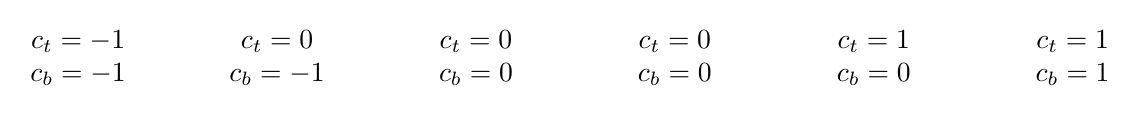
\begin{tikzpicture}[x=\linewidth/24,y=\linewidth/24]
    \drawcap{0}{nolabel}{0}{17.5}
    \coordinate (atext) at ({(0.5,7)} |- {(0.5, 7)});
    \node[anchor=south, inner sep=1pt,black,align=center] at (atext) {$c_t = -1$\\$c_b = -1$};
    \drawcap{5}{nolabel}{5.5}{17.5}
    \coordinate (btext) at ({(5.5,7)} |- {(0.5, 7)});
    \node[anchor=south, inner sep=1pt,black,align=center] at (btext) {$c_t = 0$\\$c_b = -1$};
    \drawcap{10}{nolabel}{11}{17.5}
    \coordinate (ctext) at ({(10.5,7)} |- {(0.5, 7)});
    \node[anchor=south, inner sep=1pt,black,align=center] at (ctext) {$c_t = 0$\\$c_b = 0$};
    \drawcap{15}{nolabel}{0}{11}
    \coordinate (dtext) at ({(15.5,7)} |- {(0.5, 7)});
    \node[anchor=south, inner sep=1pt,black,align=center] at (dtext) {$c_t = 0$\\$c_b = 0$};
    \drawcap{20}{nolabel}{5.5}{11}
    \coordinate (etext) at ({(20.5,7)} |- {(0.5, 7)});
    \node[anchor=south, inner sep=1pt,black,align=center] at (etext) {$c_t = 1$\\$c_b = 0$};
    \drawcap{25}{nolabel}{8.5}{14}
    \coordinate (ftext) at ({(25.5,7)} |- {(0.5, 7)});
    \node[anchor=south, inner sep=1pt,black,align=center] at (ftext) {$c_t = 1$\\$c_b = 1$};

    \drawframe{27.5}{nolabel}
  \end{tikzpicture}
\end{document}
